\documentclass[11pt,a4paper]{article}
\usepackage[utf8]{inputenc}
\usepackage{graphicx}
\usepackage[table]{xcolor}
\usepackage[overlay,absolute]{textpos}
\usepackage[multiple]{footmisc}
\usepackage{fancyhdr}
\usepackage{hyperref}
\usepackage[top=35mm, bottom=35mm, left=35mm, right=30mm]{geometry}
\usepackage[style=ieee,autocite=inline,bibencoding=ascii,backend=bibtex]{biblatex}
\usepackage{xstring}
\usepackage{caption}
\usepackage{array}
\usepackage{float}
\usepackage{setspace}
\usepackage{pdflscape}
\usepackage[number]{abstract}
\usepackage{afterpage}
\usepackage{listings}
\usepackage{algpseudocode}
\usepackage{algorithm}
\usepackage{amsmath}
\usepackage{pgfgantt}
\usepackage{subcaption}
\usepackage{pdflscape}
\usepackage{cleveref}
\usepackage{pgf,tikz}
\usepackage[australian]{babel}
\usepackage[titletoc, header, title]{appendix}
\usetikzlibrary{arrows.meta,calc} %%% Add calc


%\singlespacing
\onehalfspacing
%\doublespacing

\fancyhf{} % clear all header and footers
\rfoot{\thepage}
\pagestyle{fancy}

% For inserting a blank page.
\newcommand{\blankpage}{
\newpage
\thispagestyle{empty}
\mbox{}
\newpage
\addtocounter{page}{-1}
}

\newcolumntype{L}[1]{>{\raggedright\let\newline\\\arraybackslash\hspace{0pt}}m{#1\textwidth}}
\newcolumntype{C}[1]{>{\centering\let\newline\\\arraybackslash\hspace{0pt}}m{#1\textwidth}}
\newcolumntype{R}[1]{>{\raggedleft\let\newline\\\arraybackslash\hspace{0pt}}m{#1\textwidth}}
\newcolumntype{P}[1]{>{\raggedright\right\newline\\\arraybackslash\hspace{0pt}}p{#1\textwidth}}

%% To prevent overfull hbox in bibliography.
\emergencystretch=1em

%%% Include bibtex references.
\addbibresource{references.bib}

\graphicspath{ {./figures/} }

\title{Final Report}
\author{Taylor Young\\Student Number: 3206230}

\begin{document}
%Title
\def\isfinalreport{1}
\begin{titlepage}
    \begin{center}
        % Upper part of the page. The '~' is needed because \\
        % only works if a paragraph has started.
        \begin{center}
            \includegraphics[width=0.15\textwidth]{./figures/uon_logo.png}
            
            \textsc{\LARGE University of Newcastle}\\[1cm]
        \end{center}
        
        % Title
        % Author and supervisor
        \begin{textblock*}{133mm}(49mm,75mm)  %% change width of box from 10in as you wish
            \begin{minipage}[t][65mm][t]{133mm}
                \centering
                ~\\[0.5cm]
                \textsc{\Large Interim Report}\\[0.5cm]
            
                \hrule ~\\[0.5cm]
                { \Large Pneumatic Muscle Joint Research and Design\\[0.5cm] }
                \hrule ~\\[0.5cm]
            
                \noindent
                \begin{minipage}{0.4\textwidth}
                    \begin{flushleft} \large
                        \emph{Author:}\\
                        Taylor \textsc{Young}\\
                        Student Number: 3206230
                    \end{flushleft}
                \end{minipage}%
                \begin{minipage}{0.4\textwidth}
                    \begin{flushright} \large
                        \emph{Supervisors:} \\
                        Colin \textsc{Coates}\\
                    \end{flushright}
                \end{minipage}\\[0.5cm]
                \hrule ~\\[0.3cm]
                {\large \today}
            \end{minipage}
        \end{textblock*}
    \end{center}
    
    \vfill
    
    \emph{A thesis submitted in partial fulfilment of the requirements for the degree of Bachelor of Engineering in Electrical (Computer or Telecommunications) Engineering at The University of Newcastle, Australia.}
    
    \vfill
\end{titlepage}

% pdflatex -synctex=1 -shell-escape Final_Report.tex
\blankpage
\pagenumbering{gobble}

%%% Use roman numerals for page numbering in document preamble (abstract, TOC, acknowledgements, etc).
\pagenumbering{roman}

%Abstract
\section*{Abstract}
\addcontentsline{toc}{section}{Abstract}
Humanoid robotics is a fast-developing field encompassing a wide range of engineering disciplines to solve the challenges of robotics interaction in an environment designed for humans. In order to encourage this development many competitions exist around very common but highly specific human tasks, all of which aim to extend the field of humanoid robotics and general intelligence. In order to walk, robots need some method of actuating joints in a controllable, fast and energy efficient way.\newline
This project is to design and construct a single leg based on a custom developed humanoid robotic platform, focusing on the knee and ankle joints specifically. A single degree of freedom test rig has been constructed to test the feasibility of both the pneumatic muscles and the control scheme.
A mathematical model for the actuator has been used to inform the control system structure and allow the estimation of the current system state. Pneumatic muscles are a highly nonlinear actuator, this means that standard linear controllers have limited success in controlling the actuator position. Control can be achieved with only a static force map leading to an accurate, high-performance control scheme, however, pneumatic muscles also have their own dynamics, like hysteresis, some thermodynamic effects. \newline
Therefore, a nonlinear MPC controller has been implemented and theoretically compared to two other controllers. \newline \newline TODO This probably needs more about muscle design
\blankpage

% %Acknowledgements
% \section*{Acknowledgements}
\addcontentsline{toc}{section}{Acknowledgements}
\raggedright\hfill\break

This project has been made possible by a number of people and it is my pleasure to convey my appreciation to them in this acknowledgement.\newline

I would like to express my gratitude to my academic supervisor, Colin Coates. Without Colin's invaluable expertise, encouragement, patience and support, this project would not have been possible. His guidance throughout the year has allowed me to spend my time effectively, enhancing the focus of the work produced. I could not have completed this without his guidance.\newline

In addition to my supervisor, I would like to thank the other academics and lab staff who have provided much assistance throughout my degree. Specifically Phillip Dombkins, without Phillip much of the research and development of pneumatic muscles would not have been possible.\newline

My thanks also goes to NUbots which has provided me invaluable experience
throughout my degree. The experience gained through the variety of humanoid robotic projects has given me an insight and passion for the field, and provided part of the inspiration to undertake this project.\newline

I would also like to thank my fellow students for the stimulating discussions, brainstorming
sessions, encouragement and company during the numerous sleepless nights working towards
deadlines over the course of this degree.\newline

Last but certainly not least, I would like to thank my family and friends for their love and
support throughout my life, and in particular, this very challenging year.
% \blankpage

% %Contributions
% \section*{Contributions}
\addcontentsline{toc}{section}{Contributions}

The project described in this thesis is based in the discipline of Computer Science. The key contributions to this project are listed below:

\begin{itemize}
    \item List significant contributions
\end{itemize}

\raggedright\hfill\break\vfill

\noindent\begin{tabular}{ll}
    \makebox[2.5in]{\hrulefill} & \makebox[2.5in]{\hrulefill}\\
    Alex Biddulph & Date\\[8ex]% adds space between the two sets of signatures
    
    \makebox[2.5in]{\hrulefill} & \makebox[2.5in]{\hrulefill}\\
    Shamus Smith & Date\\
\end{tabular}


% \blankpage

%Contents
\tableofcontents
\newpage

%%% Use arabic numbers for page numbering in report body.
\pagenumbering{arabic}

\section{Introduction}
\label{sec:introduction}
\subsection{Motivation}
\label{sub:motivation}

Humanoid robotics is a fast-developing field encompassing a wide range of engineering disciplines to solve the challenges of robotics interaction in an environment designed for humans. In order to encourage this development many competitions exist around very common but highly specific human tasks, all of which aim to extend the field of humanoid robotics and general intelligence. Robocup \cite{kitano1995robocup}, is just one example of a competition utilising a simple soccer game as the platform for the research and development of humanoid robots. Robocup involves teams of robots attempting to play a game of soccer on a scaled soccer field. Whilst this may seem trivial, in order to play soccer, you need the ability to perform three major tasks. These three tasks consist of vision, localisation, and locomotion. Vision is used to locate objects in the world, balls, goals, field lines and obstacles. This system is forms the majority of the input into the system, this information is then used to determine the action to take. Localisation is responsible for determining whether the information is correct and consistent with the previous input data, filtering this information into what the robot perceives as the current world state. The last major system, locomotion, then allows the robot to move about the world to some desired location determined by the behaviour system. In order to perform this task, the robot needs some method of actuating joints in a controllable, fast and energy efficient way. Currently, actuators used by different humanoid league teams are limited to two main products, dynamixel servos \cite{robotis_mx106} or custom designed servo motors. These are both expensive and are limited in the speed and torque which can be output from the actuator. Major leaders in the field of humanoid robotics and robotics mostly use hydraulics \cite{atlas}, this allows them to carry larger payloads and run for longer periods of time. However, this also has it's trade offs increasing the weight of the platform and the speed in which it can move. \newline

Thus the motivation for this project is to design can construct an alternate actuator capable of out performing the currently used actuators as far as the speed, energy efficiency and torque in which it can perform. 

\subsection{Overview}
\label{sub:overview}

This project is to design and construct a single leg based on a custom developed humanoid robotic platform, focusing on the knee and ankle joints specifically. A mathematical model for the actuator will be used to inform the control system structure and allow the estimation of the current system state. The performance criteria for the actuator will be compared against two currently used dynamixel servos, the \cite{robotis_mx106} and \cite{robotis}.

\newpage
\subsection{Outline}
\label{sub:outline}
\begin{enumerate}
\item \textbf{Related Work} The current research relevant to the specified project broken into three major areas. The design and construction of functioning pneumatic muscles, control methods used to control linear and non linear systems, and methods of modelling static and dynamic systems. The construction of pneumatic muscles consist of an outer braided mesh and inner rubber or latex bladder, at one end the bladder has an air tight seal with the braided mesh fixed in place and at the other it contains an inlet for the compressed air. A muscle model can be divided into two main parts, mechanical and pneumatic, a model can be described in terms of its static relationships between forces using methods such as finite element analysis or virtual work relationships \cref{sub:staticforcederive}. These models can be extended by considering more complex dynamic characteristics of the system.
\item \textbf{System Implementation} This project specifically aims to design and construct a knee and ankle joint for a single leg, this will form the basis for the proposed humanoid robotic platform. The knee joint will consist of a pair of muscles acting as the flexion and extension muscles.  These will be placed on the upper leg area of the robot. To achieve the 2 DoF dorsiflexion/plantar flexion and eversion/inversion of the ankle, 2 pairs of coupled muscle actuators will be placed around the lower leg.
\item \textbf{Testing and Evaluation} Whilst attempting to perform these tests the actuators designed an implemented showed  a  less  than  desirable  lifetime  for  inflation/deflation  cycles.   Three  actuators failed within 10 cycles of inflation.  This is expected to be due to an incompatibility between the inner bladder and the braided mesh as described in [11].  Moving forward different  bladders  will  be  tested  to  determine  an  effective  compatibility  combination by  varying  the  material,  diameter  and  thickness  of  the  selected  bladder.
\item \textbf{Conclusion} This chapter is a summary of the current progress in the project.
\item \textbf{Further Work} The second phase of the project as outlined in \cref{sub:gantt_chart} consists of four major stages, the development of a static force map, evaluation of a step response, design and construction of the ankle and knee joints, and development of a model based control scheme.
\end{enumerate}

\newpage
\section{Related Work}
\label{sec:related_work}

The follow chapter outlines the current research relevant to the specified project. This project can be defined into three major areas, the design and construction of functioning pneumatic muscles, control methods used to control linear and non linear systems, and methods of modelling static and dynamic systems. 

\subsection{Pneumatic Muscles}
\label{sub:pneumatic_muscles}
Pneumatic air muscles have many names fluidic muscle, pneumatic muscle actuator, air muscle, axially contractible actuator, tension actuator, fluid actuator and fluid driven tension actuator \cite{najmuddin_mustaffa_2017} \cite{lau_chai_2012}. These are often shortened to PAM (pneumatic air muscle) or PMA (pneumatic muscle actuator) and are used interchangeably throughout research. PAM were first developed under the name McKibben Artificial Muscle in the 1950s for use in prosthetic limbs, they were then commercialised by the Bridgestone rubber company in the 1980s under the name Rubbertuators. Since then two major companies have developed PAMs for commercial purposes, Festo and the Shadow Robot Company. As \cref{fig:pneumatic_design} shows, the construction of pneumatic muscles consist of an outer braided mesh and inner rubber or latex bladder, at one end the bladder has an air tight seal with the braided mesh fixed in place and at the other it contains an inlet for the compressed air. PAM typically require external sensing mechanisms due to their nonlinear behaviours; these often measure pressure, axial contraction and exerted force of the actuator \cite{erin_pol_valle_park_2016}. \newline

Pneumatic muscles are the biological motor for locomotion or manipulation with advantages like the passive damping, good power to weight ratio, low maintenance, low price and usage in rough environments \cite{ranjan_upadhyay_kumar_dhyani_2012}. They are ideal for use in human environments in applications of human interaction such as rehabilitation therapy, nursing elderly people, and day to day work support for elderly people \cite{saga_nagase_saikawa_2006}. Compared to traditional actuators in the form of electric servos, pneumatic muscles are highly nonlinear requiring complex controllers to perform precise movements. \newline

\begin{figure}[hbt!]
    \centering
    \caption{Pneumatic Muscle Actuator Design \cite{pneumatic_image}}
    \includegraphics[scale=0.6]{Pneumatic-Muscle-Actuator-Design.png}
    \label{fig:pneumatic_design}
\end{figure}

Previous studies have looked at alternate sensing methods utilising self-contained displacement and force sensors removing the requirement for external sensing elements that allow the detection of axial contraction force and displacement at the same time. Traditionally linear encoders and load cells have been used to fulfil this task increasing the devices form factor and reducing compliance. Existing solutions include dielectric elastomers, embedded microfluidic elastomers, conductive fibre mesh and inductive coils all of which use changing resistance or inductance to measure the displacement. These mechanisms often require special manufacturing processes that limit the selection of the elastomer \cite{erin_pol_valle_park_2016}. 
Additionally, research has focused on the compatibility between the braided mesh and the inner bladder. The suitability of the mesh is significant, using the optimum size braided mesh can lead to maximum contraction. Typically, PMA technology provides a maximum contraction of 25-30\% stroke compared to the 50-70\% stroke of the biological muscle \cite{andrikopoulos_nikolakopoulos_2017}. However, when the component dimensions are optimised contraction up to 51.85\% can be achieved \cite{najmuddin_mustaffa_2017}. Incompatibility of the braided mesh with the bladder forms stress regions where the bladder non-uniformly expands. When this happens, the energy is lost, and the contraction percentage is reduced. \newline

The force generated by the pneumatic muscle is dependent on the air pressure, nominal length, contraction ratio and material properties. When the air pressure rises, the muscle circumference increases while its length decreases, causing an increase in the muscle contraction. The resulting pulling force, acting in the axial direction, corresponds to the stresses in the flexible mesh. By controlling pressure, it is possible to control the pulling force and the contraction ratio of the pneumatic muscle. \newline

In order to control the flow of air in and out of the actuator an electrically controlled pneumatic proportional/servo valve can be used to adjust the flow of air. Whilst a proportional valve provides the best continuous flow behaviour, these are expensive, and to control a single muscle would require one on the input and one on the output. To supplement these valves the use of on/off solenoid 3-way 3 port valves can be used, these often are controlled via a pulse width modulation (PWM) signal to approximate proportional valves. However, this frequent valve switching can lead to shorter valve life, reducing the viability of these valves \cite{zhang_bone_2018}. In order to reduce excessive valve switching a sliding-mode control (SMC) algorithm with three operating modes can be implemented ensuring the valves switch only when it is necessary for the desired closed-loop performance. This will be discussed in further detail in the control section of this paper \cref{sub:sliding_mode_control}. \newline

Numerous studies have been presented into the feasibility of various robotic platforms based around the use of pneumatic muscles. Humanoid Robotic Leg (HURL) was a conceptual 10 degree of freedom (DOF) lower-limb humanoid platform that was a bio-metrically informed mechanical design that attempted to improve biped robots. This research only implemented the ankle joint concluding that a more complex control structure for torque and compliance control was required, utilising a dynamic model for increased performance \cite{andrikopoulos_nikolakopoulos_2017}. Similarly, a quadruped robot driven by Festo air muscles was designed to be a test bed for the implementation and control of pneumatic muscles in legged locomotion. This work suggests the inclusion of a model for the Festo air muscle that incorporates the kinematics of the platform should be implemented in future works \cite{aschenbeck_kern_bachmann_quinn}. Anthropomorphic robotic hand designs have also been designed with the goal of achieving basic human hand grasps. These use nylon tendon-like cables to transmit the power from a forearm section containing the muscles to the end effectors making them suitable for delicate object manipulation \cite{lau_chai_2012}.

\subsection{Control Methods}
\label{sub:control_methods}
As mention in \cref{sub:pneumatic_muscles}, pneumatic muscles are a highly nonlinear actuator, this means that standard linear controllers have limited success in controlling the actuator position. Often it is possible to linearise a nonlinear plant around some known operating region in order to implement linear control structures. This could be utilised to control pneumatic muscles if the response curve of the actuator had a useful near linear region to linearise about, however, as seen later in \cref{sub:system_modelling} this is not the case and thus a controller designed to handle nonlinear properties should be used. 

\subsubsection{ANPID}
\label{sub:pid}
Advanced nonlinear proportional integral differential (ANPID) controllers are an extension of a linear control structure (PID) that attempts to provide an advanced, flexible and adjustable control performance for custom applications, without requiring knowledge of the setups model. These can be difficult to fine tune the control parameters to achieve efficient control performance and can require an additional layer to schedule gains of the system according to the operating regions and movement type \cite{andrikopoulos_nikolakopoulos_2017}. This scheme lends itself to applications where the system dynamics are unknown and difficult to measure. Generally, this isn't a restriction faced when developing a platform from the ground up and thus implementing a control structure that has an increased knowledge of the system dynamics should be used.

\subsubsection{Model Predictive Control}
\label{sub:model_predictive_control}
%%% Alex: If MPC is known as a good way to handle non-linear control, then yes you should include this. Even if you dont 
%%% Alex: intend to use it, you should explain why you have discounted this method in favour of another method.
%%% Alex: You should definitely include it if there are any other PMA works that have used MPC.
%%% TODO Should this section be included with a lack of research into this topic
Model predictive control is a method for dealing with multi-variable control problems. It aims to choose a control state by solving the system state model repeatedly, with the goal of minimising the error function into the future horizon. The behaviour is based on a plant model and is highly dependant on the accuracy of this model. Model predictive control is a broader term used to cover a variety of linear and nonlinear control stuctures including Kalman and Unscented Kalman Filters.

\subsubsection{Sliding Mode Control}
\label{sub:sliding_mode_control}
As mention previously sliding-mode control (SMC) is an algorithm for controlling the position of a pneumatic cylinder by directly switching four on/off solenoid valves. SMC is used to provide superior performance in terms of valve switches per second (SPS), steady state error (SSE), setting time and overshoot. These valves are much less expensive than the proportional/servo style valves, however, have a discontinuous flow behaviour making smooth and precise position control more difficult to achieve. While PWM may be used with on/off valves to approximate proportional valves, this frequent switching reduced the lifetime of the valve \cite{zhang_bone_2018}. \newline
This algorithm known as SMC or three-mode sliding mode control (SMC3) can be extended to operate with seven regions of control (SMC7), with the goal of reducing the number of valve SPS. The mode producing the larger acceleration should be chosen since it will reduce the tracking error faster. By adding integral action to these existing algorithms, a reduced settling time and SSE can be achieved if properly applied. Furthermore, by bounding this integral action anti-windup is achieved reducing overshoot and settling time. These extended controllers are referred to as ISMC3 and ISMC7 and can reduce the SPS by up to 37\% when compared to the original SMC implementation whilst maintaining the position tracking error \cite{zhang_bone_2018}.

\subsection{System Modelling}
\label{sub:system_modelling}
The modelling of a multi-variable system allows current input values to predict future values of the output. This can be combined with real world system measurements to accurately create an error signal proportional to the system error. A muscle model can be divided into two main parts, mechanical and pneumatic, a model can be described in terms of its static relationships between forces using methods such as finite element analysis or virtual work relationships. These models can be extended by considering more complex dynamic characteristics of the system.

\subsubsection{Static Modelling}
\label{sub:static_modelling}
Most robotic systems driven by PMAs required an underlying torque controller. This can be achieved with only a static force map leading to an accurate, high-performance controller scheme. Nevertheless, a model describing the static PMA force precisely is crucial for the accuracy of the torque controller \cite{martens_boblan_2017}. Several fundamental models for PMA have been proposed to this date aimed at describing the static characteristics of PMA, approaches include functions based on energy conservation assuming the ideal cylinder nature of the muscle. These form simplified static models considering some simple structural parameters. These lumped parameter models account for the pneumatic circuit pressure and mass flow \cite{chou_hannaford_1996}. Other methods used to determine static characteristics use the isobaric, isotonic and isometric nature of a pressure dependant system. Isotonic characteristics determine the muscle length when the load is constant and there are changes in internal pressure. The isometric condition occurs when controlling the internal pressure to achieve constant contraction with a varying load. Lastly the isobaric characteristics corresponding to an axial contraction with constant pressure and a varying load \cite{takosoglu_laski_blasiak_bracha_pietrala_2016}. These principles can be used to determine formulae defining the minimum, maximum and relative static contraction. \newline

\begin{figure}[hbt!]
    \centering
    \caption{Force vs. pressure vs. length with initial length 280mm and diameter 20mm}
    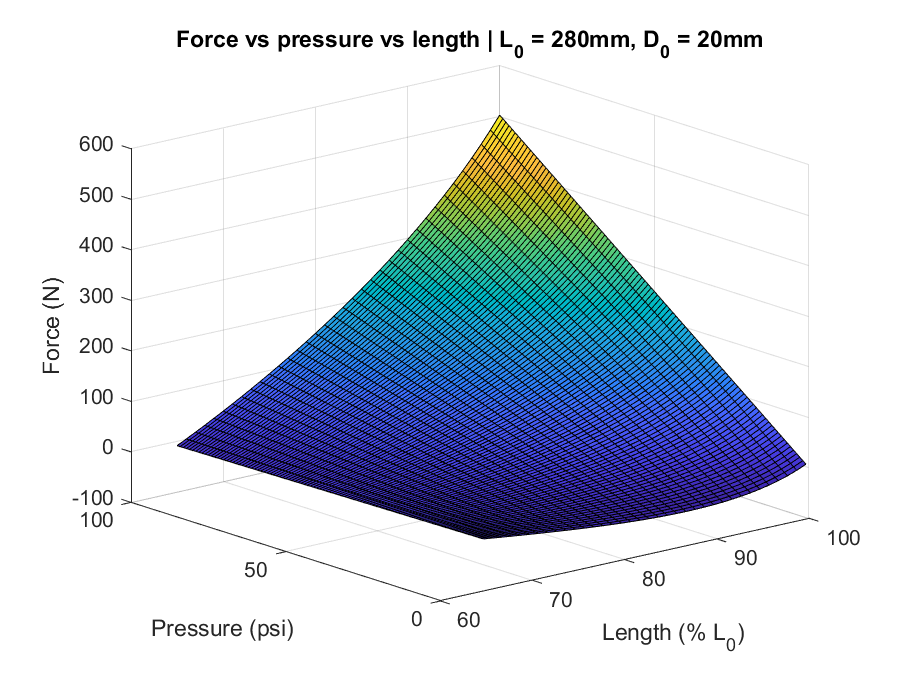
\includegraphics[scale=0.6]{staticmap.eps}
    \label{fig:staticmap}
\end{figure}

By considering both the pneumatic air compression modelling approach and the mechanical spring with varying stiffness approach, one can determine a physically motivated model that is closer to the measure force characteristic of a PMA than any existing model. The idea is the approximation of a PMA as a piston with a virtual, pressure dependent piston area and a spring that counteracts the expansion. This approach has been compared to existing models resulting in the maximum error between the new model and the measured data below 4.4\% \cite{martens_boblan_2017}. This model can be represented by a 3D static force map \cref{fig:staticmap} as a function of the pressure internal to the system and the length or contraction percentage. As seen in \cref{math:staticforce} the force generated is only dependent on the work done by the volume of air and the elasticity of the membrane, see Appendix \cref{sub:staticforcederive} for the derivation.

\begin{equation}
F_{PMA}(\rho, l) = -\rho.\frac{dV}{dL}+F_{PE}.\frac{dD}{dL}-F_L
\label{math:staticforce}
\end{equation}

\subsubsection{Dynamic Modelling}
\label{sub:dynamic_modelling}
Pneumatic air muscles have their own dynamics, like hysteresis, some thermodynamic effects and can even be interpreted as a mass spring damper combination \cite{martens_boblan_2017}. Models dependent on the construction parameter and air pressure have been developed providing a tensile force formula of the contractor actuator and can be modified to describe the extension force. One model based on a combination of sigmoid functions representing the force output as a function of both the air pressure and initial length, is an estimation derived from three experimental results over varying lengths. This model assumes an average extension ratio of 50\%, the perfect cylindrical shape with zero wall thickness of the inner bladder, constant friction-less contact between the braid and inner tube, constant braid strand length and elasticity of the rubber tube. This model lacks an accurate description of the complex non-cylindrical shape at low pressures and the imperfect contact between the inner tube and braided sleeve \cite{al-ibadi_nefti-meziani_davis_2018}. \newline

Extending this the problem can be approached firstly as a mechanically derived nonlinear spring, the stiffness of which can be controlled by the muscle pressure. This relationship can be depicted by a fifth order polynomial of two variables of 21 coefficients. The pneumatic part of the model is divided into two main components, the model of volume flow rate through the valves and a differential equation for the muscle pressure. The use of on/off style solenoid valves simplifies the flow rate to either a constant compressor pressure or atmospheric pressure, solely dependent on the muscle pressure. The second pneumatic component is the derivative time dependent equation derived from ideal gas laws. This research found that the hysteresis effects of the muscle actuator cause some steady state error due to simplified descriptions of the mechanical force components. Refinement of the model could decrease the errors to reduce the reliance on the robustness of the control technique \cite{hosovsky_2012}. Below is the equation found representing these forces \cref{math:dynamicforce}, where m - moving mass (kg), y - muscle displacement (m), F\textsubscript{S}(k,P\textsubscript{m}) - nonlinear term representing a variable spring force (N), F\textsubscript{D}(\.{k},P\textsubscript{m}) - nonlinear term representing a variable damper force (N), F\textsubscript{E} - external force (N), k - muscle contraction (defined as k = k\textsubscript{0} + y/l\textsubscript{0} where k\textsubscript{0} is the initial contraction and l\textsubscript{0} is the initial muscle length (-) and P\textsubscript{m} - the absolute muscle pressure (Pa).

\begin{equation}
    \ddot{y} = \frac{1}{m}[F_E-F_S(k,P_m)-F_D(\dot{k},P_m)]
    \label{math:dynamicforce}
\end{equation}

\newpage
\section{System Implementation}
\label{sec:system_implementation}

\subsection{Platform Design}
\label{sub:platform_design}
The ultimate goal of this design, dubbed PNEUbot, will be to develop a humanoid robotic platform designed to replicate the motions of a human closer than the current electric servo driven humanoid robots. To achieve this goal an alternate actuator must be developed, and a platform feasibility study performed to determine the viability of the actuator developed. Shown in \cref{fig:platform} this platform has been designed to mimic the range of joint movements capable by a human, this biologically inspired platform is formed around the skeleton dimensions of an adult human, implementing muscle groups to control the joints for each degree of freedom. Due to the reduced contraction of pneumatic muscles 25-30\% compared to the 50-70\% stroke of a human muscle, design constraints needed to be placed on some DoF for the range of motion available for that joint. Consequently, due to the force curve produced by pneumatic muscles, the force capable of being produced at the end of a muscle stroke is limited by its physical parameters. This project specifically aims to design and construct a knee and ankle joint for a single leg, this will form the basis for the platform.\newline

The current world class strictly humanoid robotic platform was designed by a German team from the University of Bonn. This platform stands 135cm tall, weighs 18kg and has 18 DoF: 5 per leg (parallel kinematics), 3 per arm and 2 in the neck \cite{ficht_farazi_brandenburger_rodriguez_pavlichenko_allgeuer_hosseini_behnke_2018}. These servos can produce 12.9 N.m of stall torque with a maximum rpm of 37 at no load at a 12-bit resolution \cite{robotis}. For this project, this platform will be the benchmark for the use of pneumatic air muscles as an alternate actuator. \newline

\begin{figure}[hbt!]
    \centering
    \begin{subfigure}[t]{0.4 \textwidth}
        \centering
        \caption{Side Profile}
        \includegraphics[scale=0.2]{Leg_Render_Side_2.PNG}
        \label{fig:platform_side}
    \end{subfigure}
    \begin{subfigure}[t]{0.4 \textwidth}
        \centering
        \caption{Design Concept}
        \includegraphics[scale=0.2]{Leg_Render.PNG}
        \label{fig:platform_angle}
    \end{subfigure}
    
    \definecolor{blue_m}{RGB}{83, 106, 212}
    \definecolor{mustard_m}{RGB}{200, 119, 109}
    \definecolor{sausage_m}{RGB}{197, 140, 18}
    \begin{tikzpicture}[show background rectangle,inner frame sep=2mm, scale=0.5]
        \node [fill=blue_m, rounded corners, inner sep=0.3cm, draw, thick] (A) {};
        \node [right = 0.2cm of A] (A_text) {Ankle};
        \node [right = 1cm of A_text, fill=mustard_m, rounded corners, inner sep=0.3cm, draw, thick] (B) {};
        \node [right = 0.2cm of B] (B_text) {Hip};
        \node [right = 1cm of B_text, fill=sausage_m, rounded corners, inner sep=0.3cm, draw, thick] (C) {};
        \node [right = 0.2cm of C] (C_text) {Knee};
    \end{tikzpicture}
    \caption{PNEUbot Robotic Platform Concept Design}
    \label{fig:platform}
\end{figure}

To achieve a lightweight skeleton the robot will be constructed from aluminium extrusion 'bones', 3D printed mounts and protective covers. Bearings will be inserted into the knee joint, with a spherical ball joint forming the ankle pivot. High tensile nylon line will act as tendons providing the transmission of the pneumatic muscle force to the actuated joint. \newline

The knee joint will consist of a pair of muscles acting as the flexion and extension muscles. These will be placed on the upper leg area of the robot producing approximately 120$^{\circ}$ of motion. To achieve the 2 DoF dorsiflexion/plantar flexion and eversion/inversion of the ankle, 2 pairs of coupled muscle actuators will be placed around the lower leg. These muscles will be coupled as opposed to decoupled to provide a parallel actuation force for the plantar flexion of the ankle joint. This should theoretically reduce the force required from each muscle and thus the size of the muscles contained in the lower leg. 

\subsection{Muscle Construction}
\label{sub:muscle_construction}

The pneumatic muscles are constructed from two major components, the inner bladder and the outer braided mesh. The inner bladder was chosen with an internal diameter of 6mm and wall thickness of 1.5mm, this is due to the availability and cost factors for initial testing and will likely be increased. The braided mesh of 20mm diameter was selected to be compatible with the bladder diameter as according to \cite{andrikopoulos_nikolakopoulos_2017}.

\subsection{Pneumatic Control}
\label{sub:pneumatic_control}

In order to control the flow of air into and out of the muscle bladder a 3 port 2-way pneumatic solenoid valve was used in conjunction with a non-return valve \cite{airsky_pneumatic}. These components were assembled as shown in \cref{fig:pneumatic_valve}, this arrangement allows each muscle to be in 1 of 2 states which some transitions states occurring.

\begin{figure}[hbt!]
    \centering
    \caption{Single Muscle Actuator Assembly}
    \scalebox{0.5}{
        \begin{tikzpicture}
            % Left half
            \draw[very thick] (0, 0) rectangle (5, 5);
            \draw[very thick,black,-{Triangle}] (1.25, 0) -- (1.25, 5);
            \draw[very thick,black] (3.75, 0) -- (3.75, 1);
            \draw[very thick,black] (3.25, 1) -- (4.25, 1);
    
            % Right half
            \draw[very thick] (5, 0) rectangle (10, 5);
            \draw[very thick,black,-{Triangle}] (6.75, 5) coordinate (A) -- (8.75, 0) coordinate (R);
            \draw[very thick,black] (6.25, 0) -- (6.25, 1) coordinate (P);
            \draw[very thick,black] (5.75, 1) -- (6.75, 1);
            \draw[very thick,black] (8.75, 0) -- (8.75, -1);
            \draw let \p1=(P), \p2=(A) in (\x1, \y2) node[below] {\Large{A}};
            \draw (P) node[above] {\Large{P}};
            \draw let \p1=(P), \p2=(R) in (\x2, \y1) node[above] {\Large{R}};
    
            % Right coil
            \draw (10, 1.5) -- (10.5, 3.5) -- (11.0, 1.5) -- (11.5, 3.5) -- (12.0, 1.5) -- (12.5, 3.5);
            \draw (0, 6) node[right] {\LARGE{Solenoid Valve}};
    
            % Non-return valve
            \draw let \p1=($(P) - (0, 4)$) in (\p1) circle (1);
            \draw let \p1=($(P) - (1.5, 4)$), \p2=($(P) + (1.5, -4)$), \p3=($(P) - (0, 5.5)$) in (\p1) -- (\p3) -- (\p2);
            \draw let \p1=($(P) - (0, 3)$), \p2=($(P) - (0, 2)$) in (\p1) -- (\p2);
            \draw let \p1=($(P) - (0, 5.5)$), \p2=($(P) - (0, 6.5)$) in (\p1) -- (\p2);
            \draw let \p1=($(P) + (1.5, -4)$) in (\p1) node[right] {\LARGE{Non-return Valve}};
    
            % Muscle
            \coordinate (pole) at (20, -5);
            \foreach \i in {1,...,20}
            {
                \draw[very thick] let \p1=(pole) in (\x1, \y1 + \i * 20) -- (\x1 + 80, \y1 + \i * 20 - 25);
            }
            \draw[very thick] let \p1=(pole) in (\x1, \y1 - 5) rectangle (\x1 + 80, \y1 + 20 * 20);
            \draw let \p1=(pole) in (\x1 + 90, \y1 + 200) node[right] {\LARGE{Pneumatic Air Muscle}};
    
            % Bottom cap
            \draw[very thick] let \p1=(pole) in (\x1 - 10, \y1 - 5) rectangle (\x1 + 90, \y1 - 25);
            \draw[very thick] let \p1=(pole) in (\x1, \y1 - 25) arc (180:360:1.4);
    
            % Top cap
            \draw[very thick] let \p1=(pole) in (\x1 - 10, \y1 + 20 * 20) rectangle (\x1 + 90, \y1 + 20 * 20 + 20);
            \draw[very thick] let \p1=(pole) in (\x1, \y1 + 20 * 20 + 20) arc (180:0:1.4);
            
            % Line from solenoid valve to top of muscle
            \draw[very thick] let \p1=(A), \p2=(pole) in (\x1, \y1)[rounded corners=10pt]{} --
              (\x1, \y2 + 20 * 20 + 100){} --
              (\x2 + 40, \y2 + 20 * 20 + 100){} --
              (\x2 + 40, \y2 + 20 * 20 + 60){};
    
            % Line from non-return valve to solenoid valve
            \draw[very thick] let \p1=($(P) - (0, 2)$) in (\x1, \y1) -- (P);
    
            % Input line
            \draw[very thick] let \p1=($(P) - (0, 6.5)$), \p2=($(P) - (0, 10)$) in (\x1, \y1) -- (\x2, \y2) node[midway,label=right:{\LARGE{Regulated Air In}}]{};
        \end{tikzpicture}
    }
    \label{fig:pneumatic_valve}
\end{figure}

Consider one muscle under no load when its internal pressure is equal to the regulated system pressure, the muscle will be under full contraction. Releasing the air from the muscle will allow the muscle to extend back to its nominal length. Switching between the two valve states will allow the muscle to contract and release. Now consider the case where two muscles of equal parameters are appended end to end. Starting with both muscles at equilibrium pressure, regulated system pressure, the contraction percentage of both muscles will be equal. Switching the first muscle into the open position will allow the air to release from that muscle, this also allows the second muscle to contract filling with air. When the required position is reached the first muscle can be switched closed, causing the muscle to re-pressurise stopping the contraction of the second muscle. If the non-return valve was not installed, the system would be able to equalise the pressure between the two muscles when the force generated by each muscle was different due to the different contraction percentages. These states are like the SMC3 modes, however, the use of two valves per pair of muscles instead of four reduces the cost of the valves for the system. This also means that a SMC7 implementation is not possible, due to the limited number of states that the valve positions can form.
Each valve is controlled by the circuit described in \cref{sub:shield} by the micro controller \cref{sub:microcontroller}.

\subsection{Sensors}
\label{sub:sensors}
To measure the states of the system, pressure and linear position, a pressure sensor and linear potentiometer have been chosen. The pressure sensor is placed after the valve on the muscle side of the actuator. This pressure sensor \cite{NBPLANN100PGUNV} allows readings from 0 to 100 psi and was attached to a custom PCB that provides a differential reading of the sensor to be fed into the micro controller. A rotary potentiometer or encoder could have been used for the axial position measurement and placed on the rotational axis of each joint, however, the design and construction for the 2 DoF ankle joint would be more complex. This then lends itself to the use of linear potentiometers attached to the end of each muscle, eliminating the need to a sensor attached directly to the rotational axis. This solution directly reads the contraction distance of the muscle rather than the ankle of the joint, requiring some knowledge of the robot kinematics to calculate the angular position.

\subsection{Micro controller}
\label{sub:microcontroller}
For an entire PNEUbot leg with 6 DoF, a total of 12 muscles would be needed to achieve the required movement. This in turn would require 24 sensor inputs to read the pressure and position of each muscle. This requires a micro controller that contains 24 ADC channels, one for each sensor, that can run fast enough to compute the control methods implemented and perform the sensor readings. The NUCLEO-STM32F722ZE \cite{nucleo_stm32f722ze} has 24 individual ADC channels available and runs with a maximum clock frequency of 216MHz, this micro controller should allow enough processing overhead to achieve the required task.

\subsubsection{Electronics Shield}
\label{sub:shield}
In order to control the valves and read the pressure and potentiometer sensors a PCB was designed to hold the logic level MOSFET control circuits for each valve. This board also contains a differential amplifier circuit that is driven by the pressure sensor, with breakout headers for all the external sensors. The shield plugs into the micro controller via the ST-Morpho connectors on the NUCLEO board. %% TODO Design this board... \cref{fig:shield}.

\subsubsection{Software}
\label{sub:software}
The software architecture follows the structure shown in \cref{fig:software_arch}. The system is comprised of three major subsystems, the Leg Controller, ADC, and the Joints. The first subsystem, the leg controller takes the requested leg positions via an end effector or motion command and calculates the inverse and forward kinematics to determine the angle of each joint. The second subsystem, the ADC reads in sequence each of the sensors updating the data fed into the control loop as often as possible. The third subsystem consists an instance of each joint in the system. One and two axis joints are implemented each of which contain an instance of all the muscles for that specific joint as well as a controller which takes the reference angles for the joints and drives the setpoint for each muscle. Each muscle then also contains a valve, pressure sensor and linear potentiometer associated with that muscle as well as the relevant micro controller pins. This software structure allows all muscles to contain the same base control methods with varying parameters between them.

\begin{figure}[hbt!]
    \centering
    \caption{Software architecture}
    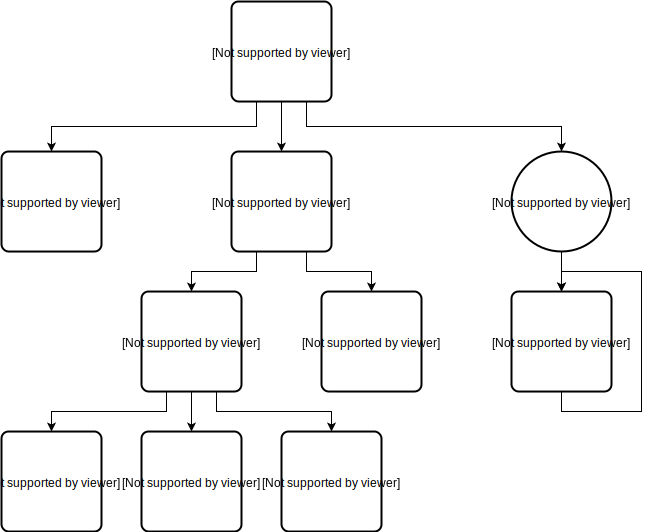
\includegraphics[scale=0.5]{Software_Arch.png}
    \label{fig:software_arch}
\end{figure}

\clearpage
\section{Testing and Evaluation}
\label{sec:results}

The initial test setup for the static map and step response consists of two muscles attached end to end mounted to a backing board. This backing board also contains a valve for each muscle and the required pneumatic hoses and fittings to provide the system pressure. Mounted between the two muscles is a linear potentiometer used to measure the position response of the step input. The valves and potentiometer are wired into the micro-controller to allow feedback of the states and positions of the devices. The system pressure has been tested to be safe up to 60 psi whilst maintaining full contraction of the pneumatic actuator.\newline

Whilst attempting to perform these tests the actuators designed an implemented showed a less than desirable lifetime for inflation/deflation cycles. Three actuators failed within 10 cycles of inflation. This is expected to be due to an incompatibility between the inner bladder and the braided mesh as described in \cite{andrikopoulos_nikolakopoulos_2017}. Moving forward different bladders will be tested to determine an effective compatibility combination by varying the material, diameter and thickness of the selected bladder. The latex bladder used was found to have inconsistent tolerances in material thickness along the length of the sample, this would result in nonuniform inflation of the bladder resulting in increased pressure and stress regions of the material.

\newpage
\section{Conclusion}
\label{sec:conclusion}

Humanoid robotics is a fast-developing field encompassing a wide range of engineering disciplines to solve the challenges of robotics interaction in an environment designed for humans. In order to encourage this development many competitions exist around very common but highly specific human tasks, all of which aim to extend the field of humanoid robotics and general intelligence. Robocup \cite{kitano1995robocup}, is just one example of a competition utilising a simple soccer game as the platform for the research and development of humanoid robots. Robotics requires three major areas of research one of which, locomotion, allows the robot to move about the world to some desired location determined by the behaviour system. In order to perform this task, the robot needs some method of actuating joints in a controllable, fast and energy efficient way. Currently, actuators used by different humanoid league teams are limited to two main products, dynamixel servos \cite{robotis_mx106} or custom designed servo motors. These are both expensive and are limited in the speed and torque which can be output from the actuator. Major leaders in the field of humanoid robotics and robotics mostly use hydraulics \cite{atlas}, this allows them to carry larger payloads and run for longer periods of time. However, this also has it's trade offs increasing the weight of the platform and the speed in which it can move. \newline

This project is to design and construct a single leg based on a custom developed humanoid robotic platform, focusing on the knee and ankle joints specifically. A mathematical model for the actuator will be used to inform the control system structure and allow the estimation of the current system state. The performance criteria for the actuator will be compared against two currently used dynamixel servos, the \cite{robotis_mx106} and \cite{robotis}.\newline

Pneumatic air muscles are referred to by many names, these are often shortened to PAM (pneumatic air muscle) or PMA (pneumatic muscle actuator) and are used interchangeably throughout research. As \cref{fig:pneumatic_design} shows, the construction of pneumatic muscles consist of an outer braided mesh and inner rubber or latex bladder, at one end the bladder has an air tight seal with the braided mesh fixed in place and at the other it contains an inlet for the compressed air. PAM typically require external sensing mechanisms due to their nonlinear behaviours; these often measure pressure, axial contraction and exerted force of the actuator \cite{erin_pol_valle_park_2016}. To measure the states of the system, pressure and linear position, a pressure sensor and linear potentiometer have been chosen. The pressure sensor is placed after the valve on the muscle side of the actuator and the linear potentiometers attached to the end of each muscle. This eliminates the need to a sensor attached directly to the rotational axis. Pneumatic muscles are a highly nonlinear actuator, this means that standard linear controllers have limited success in controlling the actuator position. Most robotic systems driven by PMAs required an underlying torque controller. This can be achieved with only a static force map leading to an accurate, high-performance controller scheme. Nevertheless, a model describing the static PMA force precisely is crucial for the accuracy of the torque controller \cite{martens_boblan_2017}. Several fundamental models for PMA have been proposed to this date aimed at describing the static characteristics of PMA, approaches include functions based on energy conservation assuming the ideal cylinder nature of the muscle. These form simplified static models considering some simple structural parameters. Pneumatic air muscles also have their own dynamics, like hysteresis, some thermodynamic effects and can even be interpreted as a mass spring damper combination \cite{martens_boblan_2017}. Models dependent on the construction parameter and air pressure have been developed providing a tensile force formula of the contractor actuator and can be modified to describe the extension force.\newline

The ultimate goal of this design  will be to develop a humanoid robotic platform designed to replicate the motions of a human closer than the current electric servo driven humanoid robots. To achieve this goal an alternate actuator must be developed, and a platform feasibility study performed to determine the viability of the actuator developed. Shown in \cref{fig:platform} this platform has been designed to mimic the range of joint movements capable by a human, this biologically inspired platform is formed around the skeleton dimensions of an adult human, implementing muscle groups to control the joints for each degree of freedom. \newline

Whilst attempting to perform these tests the actuators designed an implemented showed a less than desirable lifetime for inflation/deflation cycles. Three actuators failed within 10 cycles of inflation. This is expected to be due to an incompatibility between the inner bladder and the braided mesh as described in \cite{andrikopoulos_nikolakopoulos_2017}. Moving forward different bladders will be tested to determine an effective compatibility combination by varying the material, diameter and thickness of the selected bladder. The latex bladder used was found to have inconsistent tolerances in material thickness along the length of the sample, this would result in nonuniform inflation of the bladder resulting in increased pressure and stress regions of the material.

\newpage
\section{Further Work}
\label{sec:further}
The second phase of the project is outlined in \cref{sub:gantt_chart}, this involves four major stages as outlined below.

\subsection{Static Map}
\label{sub:static_map}
In order to compare the performance of the muscle against the theoretical models found in \cite{martens_boblan_2017} and \cite{hosovsky_2012}, a static map of the force generated at varying pressures and contraction length will be produced. This will also inform the coefficients of the surface polynomial required for the use of the dynamic model. This test will be conducted by suspending a muscle from one end with a variable mass attached to the other end. By varying the pressure, a contraction percentage can be measured and thus the static map can be generated. This static map will be compared to the ideal theoretical static map as seen in \cref{fig:staticmap}.

\subsection{Step Response}
\label{sub:step_response}
The first step to developing and evaluating a control strategy is to perform a step response of the system. This step response will form part of the performance metric for the viability of pneumatic muscle actuators for use within a humanoid robot. The step response will be conducted with a pair of muscles attached end on end and fixed to a backing plate. One muscle will begin fully contracted and the system pressure will be applied to the second. When the first muscles valve is switched, the second will contract, forming the step response curve.

\subsection{Leg Construction}
\label{sub:leg_construction}
The next stage of this project will involve the construction of the knee and ankle joints as a complete system. Construction of the remaining muscles with the finalisation of the mounting hardware required to attach each component to the leg assembly. This will require estimating the length of muscle required for each muscle group to achieve the required contraction and thus angular motion of a human.

\subsection{Model Control}
\label{sub:mpc_implementation}
The second major aspect for future work is the implementation of a model based nonlinear control scheme. This is where current research in the field has identified improvements can be made opposed to using a model independent control structure. This will build on the static and dynamic models seen in \cite{martens_boblan_2017} and \cite{hosovsky_2012} respectively. The SMC3 \cite{zhang_bone_2018} valve control method should also be used to reduce the SPS of the on/off type valves used in the system. Nonlinear control methods are still yet to be researched to determine the appropriate method for this project, however, it is expected some form of model predictive control or unscented Kalman Filter will be implemented to perform this task.

\newpage
\begin{appendices}
\section{Static Force Derivation}
\label{sub:staticforcederive}
Approximating the volume as a cylinder, the dependency of the diameter on the length can be approximated by using the Pythagoras theorem 
\begin{equation}
    D(L) = \frac{\sqrt{L_{Fibre}^2-L^2}}{n \pi}
\end{equation}
This then follows that \cref{math:diameterconst1} and \cref{math:diameterconst2} are only dependent on the initial conditions
\begin{equation}
    n = \frac{L_0\tan(\Theta_0)}{\pi D_0}
    \label{math:diameterconst1}
\end{equation}
\begin{equation}
    L_{Fibre} = \frac{L_0}{\cos(\Theta_0)}
    \label{math:diameterconst2}
\end{equation}
Inserting the functional dependency on the diameter into the equation of a cylinder results in a volume only dependent on the length and initial conditions
\begin{equation}
    V(L) = \frac{L L_{Fibre}^2}{4 \pi n^2}-\frac{L^3}{4 \pi n^2}
\end{equation}
The virtual work of the PMA can be split into two parts, the work done by the volume of air and the elasticity of the membrane 
\begin{equation}
    W_{PMA} = W_{VAE} + W_{Elast}
\end{equation}
\begin{equation}
    \sigma_{L} = E_{RU}(L) \frac{L-L_0}{L_0}
\end{equation}
\begin{equation}
    \sigma_{PE} = E_{RU}(L) \frac{D-D_0}{D_0}
\end{equation}
\begin{equation}
    W_{L} = -\sigma_{L} H_0 \pi D(L)
\end{equation}
\begin{equation}
    W_{Elast-PE} = -\sigma_{PE} H_0 L \pi
\end{equation}
Finally the following equation gives the positive pulling force exherted by the muscle
\begin{equation}
    F_{PMA}(\rho, l) = -\rho \frac{dV}{dL}+F_{PE} \frac{dD}{dL}-F_L
    \label{math:staticforcederive}
\end{equation}
\newpage

% \subsection{Appendix B}
% \label{sub:shield_design}
% % TODO - Finish PCB and insert picture
% \begin{figure}[hbt!]
%     \centering
%     \caption{PNEUbot NUCLEO shield PCB design}
%     \includegraphics[scale=0.3]{Shield_PCB.png}
%     \label{fig:shield}
% \end{figure}

% \newpage

\begin{landscape}
\section{Gantt Chart}
\label{sub:gantt_chart}
\begin{figure}[ht]
    \centering
    \advance\leftskip-4cm
    \advance\rightskip-2cm
    \includegraphics[width=1.4\textwidth]{GanttChart-crop.pdf}
    \caption{Future Work Timeline}
    \label{fig:gantt_chart}
\end{figure}
\end{landscape}
\newpage

\section{Dynamic Force Derivation}
\begin{equation}
    \ddot{y} = \frac{1}{m}[F_E-F_S(k,P_m)-F_D(\dot{k},P_m)]
\end{equation}

\begin{gather}
 F_{CE} =
 \begin{bmatrix}
    1 \\ 
    k \\
    k^2 \\
    k^3 \\
    k^4 \\
    k^5 \\
   \end{bmatrix}
 \begin{bmatrix}
    1 & P_m & P_m^2 & P_m^3 & P_m^4 & P_m^5 \\
   \end{bmatrix}
  \begin{bmatrix}
    a_{00} & a_{01} & a_{02} & a_{03} & a_{04} & a_{05} \\
    a_{10} & a_{11} & a_{12} & a_{13} & a_{14} & 0 \\
    a_{20} & a_{21} & a_{22} & a_{23} & 0      & 0 \\
    a_{30} & a_{31} & a_{32} & 0      & 0      & 0 \\
    a_{40} & a_{41} & 0      & 0      & 0      & 0 \\
    a_{50} & 0      & 0      & 0      & 0      & 0 \\
   \end{bmatrix}
\end{gather}

\begin{equation}
    F_D(\dot{k},P_m) = -RP_m\dot{k}
\end{equation}

\begin{equation}
   \dot{V_a} = \begin{cases} 
        P_1C\sqrt{\frac{T_0}{T_1}}\sqrt{1-(\frac{\frac{P_2}{P_1}-b}{1-b})^2}, & \text{if}\ \frac{P_2}{P_1} > b\\ 
        P_1C\sqrt{\frac{T_0}{T_1}}, & \text{if}\ \frac{P_2}{P_1} $\leq$ b \end{cases}
\end{equation}

\begin{equation}
    \frac{d}{dt}(\frac{P_aV_a}{V_m}) = P_a(\frac{\dot{V_a}V_m-\dot{V_m}V_a}{V_m^2}) = P_a\frac{\dot{V_a}}{V_m}-P_m\frac{\dot{V_m}}{V_m}
\end{equation}

\begin{equation}
    V_m = ak^3 + bk^2 + ck + d
\end{equation}

\begin{equation}
    \dot{V_m} = 3ak^2\dot{k} + 2bk\dot{k} + c\dot{k}
\end{equation}

Where: \newline
m - moving mass (kg)\newline
y - muscle displacement (m)\newline
$F_s(k, P_m)$ - nonlinear spring force (N)\newline
$F_d(\dot{k}, P_m)$ - nonlinear damper force (N)\newline
$F_E$ - external force (N)\newline
$k = k_0 + \frac{y}{l_0}$ - muscle contraction\newline
$k_0$ - initial muscle contraction\newline
$l_0$ - initial muscle length\newline
$P_m$ - absolute muscle pressure (Pa)\newline
$a_{xx}$ - 21 coefficient static map matrix\newline
$R$ - damping coefficient $(m^2s)$\newline
$\dot{k}$ - muscle velocity (1/s)\newline
$\dot{V_a}$ - time derivative of muscle air volume (volume flow rate through the valve) $(m^3/s)$
$P_1$ - absolute upstream pressure (Pa)\newline
$C = 2.6167x10^{-9}$ - sonic conductance $(m^3/(sPa))$\newline
$T_0$ - ambient air temperature at reference conditions (K)\newline
$T_1$ - upstream temperature (K)\newline
$P_2$ - absolute downstream pressure (Pa)\newline
b = 0.433 - critical ratio\newline
$P_a$ - atmospheric pressure (Pa)\newline
$V_a$ - volume of air in the muscle $(m^3)$\newline
$V_m$ - muscle volume $(m^3)$\newline
$\dot{V_m}$ - time derivative of muscle volume $(m^3/s)$\newline
a, b, c, d - polynomial coefficients


\newpage
\end{appendices}
% \newpage
%%% Display the bibliography.
\printbibliography
\end{document}
